% Project Planner — editable & compilable online at https://letx.app
% Compiles with pdflatex. A clean one-page project planner: milestones, a
% simple Gantt-style timeline, task board, and notes. Edit the rows below.
\documentclass[11pt]{article}
\usepackage{amsmath}
\usepackage[a4paper,margin=1.6cm,landscape]{geometry}
\usepackage[T1]{fontenc}
\usepackage{lato}
\renewcommand{\familydefault}{\sfdefault}
\usepackage[table]{xcolor}
\usepackage{colortbl}
\usepackage{booktabs}
\usepackage{tabularx}
\usepackage{array}
\usepackage{tikz}
\usepackage{enumitem}
\usepackage{hyperref}
\hypersetup{hidelinks}
\setlength{\parindent}{0pt}
\pagestyle{empty}

\definecolor{ink}{HTML}{263238}
\definecolor{accent}{HTML}{5E60CE}   % indigo
\definecolor{accent2}{HTML}{48BFE3}  % sky
\definecolor{done}{HTML}{57CC99}     % green
\definecolor{band}{HTML}{F0F0FB}
\definecolor{mist}{HTML}{6C757D}
\newcolumntype{C}{>{\centering\arraybackslash}X}

% one Gantt bar: \gbar{startcol}{spancols}{color}
\newcommand{\gbar}[3]{\tikz\fill[#3,rounded corners=2pt]
  (#1*1.0,-0.14) rectangle (#1*1.0+#2*1.0,0.14);}

\begin{document}
% ---- header ----
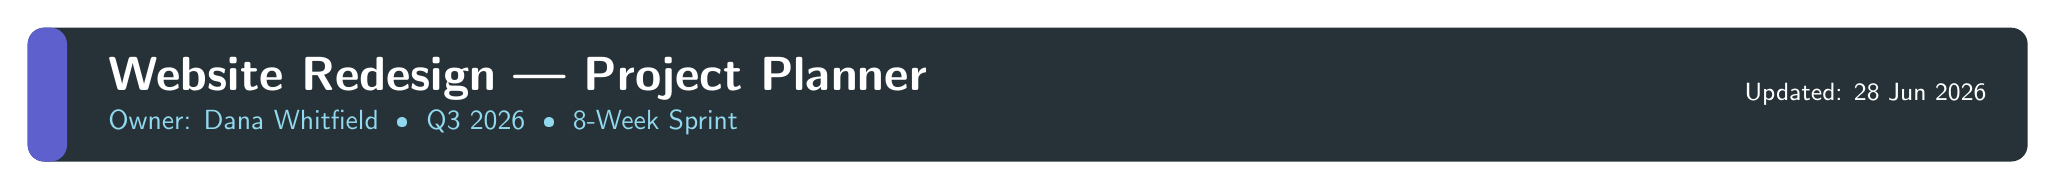
\begin{tikzpicture}
  \fill[ink,rounded corners=6pt] (0,0) rectangle (25.4,1.7);
  \fill[accent,rounded corners=6pt] (0,0) rectangle (0.5,1.7);
  \node[anchor=west,text=white,align=left] at (0.9,1.05)
    {\fontsize{18}{18}\selectfont\bfseries Website Redesign --- Project Planner};
  \node[anchor=west,text=accent2!60,align=left] at (0.9,0.5)
    {\normalsize Owner: Dana Whitfield \;\textbullet\; Q3 2026 \;\textbullet\; 8-Week Sprint};
  \node[anchor=east,text=white] at (25.0,0.85) {\small Updated: 28 Jun 2026};
\end{tikzpicture}

\vspace{0.4cm}
% ---- timeline (Gantt) ----
{\color{ink}\large\bfseries Timeline}\\[4pt]
\rowcolors{2}{band}{white}
\begin{tabularx}{\linewidth}{@{}p{4.6cm} *{8}{C} @{}}
\rowcolor{ink}
{\color{white}\textbf{Task}} & {\color{white}W1} & {\color{white}W2} & {\color{white}W3} &
{\color{white}W4} & {\color{white}W5} & {\color{white}W6} & {\color{white}W7} & {\color{white}W8}\\
Discovery \& audit   & \gbar{0}{2}{accent} &&&&&&&\\
Wireframes           && \gbar{0}{2}{accent} &&&&&&\\
Visual design        &&& \gbar{0}{2}{accent2} &&&&&\\
Front-end build      &&&& \gbar{0}{3}{accent2} &&&&\\
CMS integration      &&&&& \gbar{0}{2}{accent2} &&&\\
QA \& accessibility  &&&&&& \gbar{0}{2}{done} &&\\
Launch \& handoff    &&&&&&& \gbar{0}{2}{done}&\\
\end{tabularx}

\vspace{0.5cm}
\begin{minipage}[t]{0.46\linewidth}
% ---- milestones ----
{\color{ink}\large\bfseries Milestones}\\[4pt]
\begin{tabularx}{\linewidth}{@{}c X r@{}}
\toprule
\textbf{} & \textbf{Milestone} & \textbf{Target}\\
\midrule
\textcolor{done}{$\bullet$} & Discovery sign-off      & Jul 12\\
\textcolor{done}{$\bullet$} & Design approved         & Jul 26\\
\textcolor{accent}{$\bullet$} & Beta build ready      & Aug 16\\
\textcolor{accent}{$\bullet$} & QA complete           & Aug 23\\
\textcolor{mist}{$\bullet$} & Public launch           & Aug 30\\
\bottomrule
\end{tabularx}

\vspace{0.4cm}
{\color{ink}\large\bfseries Legend}\\[3pt]
{\small \gbar{0}{0.7}{accent}\ Design phase \quad
        \gbar{0}{0.7}{accent2}\ Build phase \quad
        \gbar{0}{0.7}{done}\ Ship phase}
\end{minipage}\hfill
\begin{minipage}[t]{0.5\linewidth}
% ---- task board ----
{\color{ink}\large\bfseries Task Board}\\[4pt]
\begin{tabularx}{\linewidth}{@{}p{2.3cm} X@{}}
\toprule
\textbf{Status} & \textbf{Items}\\
\midrule
\cellcolor{done!25}\textbf{Done} & Stakeholder interviews; content audit; sitemap\\
\arrayrulecolor{band}\midrule\arrayrulecolor{black}
\cellcolor{accent2!20}\textbf{In Progress} & Hi-fi mockups; design tokens; component library\\
\arrayrulecolor{band}\midrule\arrayrulecolor{black}
\cellcolor{band}\textbf{To Do} & CMS migration; analytics; SEO redirects; 404 page\\
\bottomrule
\end{tabularx}

\vspace{0.4cm}
{\color{ink}\large\bfseries Notes}\\[3pt]
{\small\color{mist}
Blocked: awaiting brand assets from marketing (due Jul 8). Risk: CMS migration may
slip if legacy content export is delayed --- add a 3-day buffer before launch.}
\end{minipage}

\vfill
{\color{mist}\footnotesize Made with \href{https://letx.app}{letx.app}}
\end{document}
